
%%%%%%%%%%%%%%%%%%%% file cmmr_template.tex %%%%%%%%%%%%%%%%%%%%%
%
% This is the LaTeX source for the instructions to authors using
% the LaTeX document class 'llncs.cls' for contributions to
% the Lecture Notes in Computer Sciences series.
% http://www.springer.com/lncs       Springer Heidelberg 2006/05/04
%
% It may be used as a template for your own input - copy it
% to a new file with a new name and use it as the basis
% for your article.
%
% NB: the document class 'llncs' has its own and detailed documentation, see
% ftp://ftp.springer.de/data/pubftp/pub/tex/latex/llncs/latex2e/llncsdoc.pdf
%
%%%%%%%%%%%%%%%%%%%%%%%%%%%%%%%%%%%%%%%%%%%%%%%%%%%%%%%%%%%%%%%%%%%


\documentclass[,a4paper]{llncs}

\usepackage{amssymb}
\setcounter{tocdepth}{3}
\usepackage{graphicx}
\usepackage{cite}
\usepackage{url}
\newcommand{\keywords}[1]{\par\addvspace\baselineskip
\noindent\keywordname\enspace\ignorespaces#1}

% \pagestyle{headings}
\pagestyle{empty}

\begin{document}

\mainmatter  % start of an individual contribution

\title{ArtDoc - an Experimental Archive and a Tool for Artistic Research}

\titlerunning{ArtDoc}
\author{Henrik Frisk}

\authorrunning{Henrik Frisk}
\institute{Royal College of Music in Stockholm\\ \email{henrik.frisk@kmh.se}}

\maketitle

\begin{abstract}
  ArtDoc is an experimental archive primarily for documenting artistic practice. One of the ambitions is to address the question of how artistic practice may be documented in a manner that makes visible the processes in action. ArtDoc has its roots in research and artistic practice that began over ten years ago and preliminary tests shows it to be a useful complement to other means to document musical works and artistic processes. The particular case of open form works, works that in some respect are negotiated between the different agents involved, such as composers, musicians and members of the audience was a point of departure and has guided the development to a significant degree. The underlying structure of documentation classes is presented and some of the design choices are discussed. ArtDoc is still under construction but a working proof of concept will be released in 2018.
  
\keywords{Electro acoustic music, Artistic research, Music representation, Cooperative music networks}
\end{abstract}

\section{Introduction}
What is it to document a musical work? Perhaps the most obvious way is to record the performance, but what is gained, or lost, in the transformation from the work's material reality to its recorded representation? In this paper I will attempt to approach this question indirectly by presenting a method for documenting the both the result as well as the processes behind the creation of a musical work. These thoughts have developed through my work in electro acoustic music with and without live parts in the sense that some of the particular challenges in these genres have guided the choices made.

The assumption that the process that leads up to a finished version of a work of music contains information that is valuable both for the musician performing the work and the listener that approaches the result as well as for any research activity that attempts to understand the artistic process at large, has been a guiding principle in much of the developments of artistic research in the last couple of decades \cite{biggs10}. This supposition has likewise guided much of the research in the current project and, as a consequence, whether the work is a composition, a performed improvisation or an interpretation of a musical work is less important. But however relevant the question of how to document artistic processes in music is, there is still a lack of stable solutions and tools for the requirements seen in the current project. However, several interesting and useful examples exist. One of the notable attempts to create a framework for documenting and sharing artistic research is the Research Catalogue \cite{rc2017}. Different in scope, the CASPAR project is a large scale system for archiving digital data \cite{Douglas2007,Roeder2006,Bachimont2003,cuervo2011}. These are only two out of many examples and given the impact of the process of digitization this is an area in which many new initiatives will be taken.

To add to the complexity of the question of documenting artistic practice, due to the novelty of the field of artistic research it is not always self evident what artistic research data actually consits of. Hence, even if a useful tool for documenting artistic research practice were to be developed, there is still the question of \emph{what} should be documented remains. In any research context there is a need to collect material necessary for a systematic investigation. In addition, to research processes of creation there is a need to develop a suitable method that surfaces and makes visible the activities that relate to the work creation. The issue may be divided into several subtopics but first and foremost it is important to distinguish between the gathering of research data, and the documentation of the result. As was pointed oput above, even if the result may be easily documented, the data, the processes that lead to the result, is commonly of central importance to the artistic research process. How can the integrity of the data be preserved in an artistic research project that may contain a number of different kinds of data, as well as raw material from the artistic process? 

The current research has its roots in events that started more than ten years ago, and my piece for guitar and electronics that was premiered in Beijing in 2006, \emph{Repetition Repeats all other Repetitions} \cite{friskcoessens2013}, has played an important role. Another related project that has contributed to the research to a significant degree is the \emph{Integra} project \cite{integra}. \emph{Integra} was a project hosted by Birmingham Conservatoire and funded by the EU, and one of its initial ambitions was to document electronic musical works in a sustainable manner addressing the issue that musical works that rely on technology, such as live electronic music or interactive music, may be difficult to preserve when the technology the works depend on becomes obsolete. In some cases works may become impossible to perform unless an effort is made to migrate these works to newer technologies \cite{frisk-bullock08,frisk-bull07,bullock06}. Such processes of migration are often complicated and costly and this was an experience made in the \emph{Integra} project. The overarching ambition was to collect works involving live electronics from the project partner countries and create robust and somewhat generic and technology independent descriptions of these pieces. In addition, the works adapted in the \emph{Integra} project should be documented in ways that would make it easy for musicians and music ensembles to rehearse and perform them without the composer present. It was an original ambition that all data relating to supported musical works, including scores, electronic parts, information about different versions and renderings of these works, biographical data, etc., should be stored on a web-accessible database, and that it should be possible to transfer the data to a variety of usable target applications.

Artdoc has developed out of the work done in \emph{Integra}, in particular the research that Jamie Bullock and I did concerning a hierarchy of documentation classes \cite{frisk09,frisk-bullock08}. These were to some extent influenced by the work done in the large European MUSTICA project \cite{Bachimont2003}. Whereas \emph{Integra} to a some degree had a work-centered view on the musical work, a view based on the idea that each musical work has an identity that any performer and interpreter should adhere to, the current project has the ambition to also include the processes that lead up to a performance. As such it focuses on the elements of the processes that are essential to the creation of the work and regards each instance of the work as a new configuration with new possibilities. These two models, the work-centered view and the process oriented view, obviously have very different needs when it comes to documentation, but they also overlap in interesting ways. The main empirical data is taken from my experiences with the way \emph{Repetition Repeats all other Repetitions} evolved from a strictly notated piece of music for guitar and electronics to an open form composition that has taken many shapes since its first performance.

The main difference between these two models is that in a traditional view of documentation, in which the work as it was conceived of by its originator, the performed result is actually a fairly decent means for communicating the intended result, given that the result is in line with the original intentions, and provided that there is a cultural, and perhaps social, context in which the performance took place. A good recording of a solid interpretation of a work in a known performance tradition can provide a good point of entry in the attempt to unpack its significance. However, as soon as the work questions conventional aesthetics and departs from expected traditions there is different need for contextual information in order for the work to make sense. 

This is also true in the case of a electro acoustic music where the lack of a physical performer further detaches the sonic result from the material reality of the activities that gave rise to the work. For a work for which the process of creation plays a conceptually important part, the situation is not only aesthetically substantially different, it is also philosophically different. The work's authenticity lies no longer in the intentions of the originator, but rather in the ears of the listener, or in the hands of the interpreter.\footnote{This discussion could be expanded significantly and it may well be argued that also traditional music is molded by the listener as well as the originator. See \cite{frisk-ost06-2} for an introduction.} How is such a work best documented?

ArtDoc has evolved out of this background to provide a preliminary solution to the question of how to document artistic practice in a way that allows it to be communicated to others. An important aspect of the documentation strategy discussed here is that it should also serve methodological needs of an associated artistic research effort. In order to successfully attempt to research one's own artistic practice there is a constant need to both archive the intermediary results and make connections between these and the final results. In a relatively early study in the development of creative technologies for music production Folkestad, Lindstr{\"o}m and Hargreaves showed the importance of mapping the changes in the ongoing creative process as a method for researching processes of computer-based composition \cite{Folkestad1997}. By collecting consecutive versions of the developing work by young composers they could effectively analyze the compositional strategies employed by the participants of the study.

For the rest of this short paper I will mainly discuss ArtDoc from the point of view of my own artistic work, but it nonetheless rests on the experiences and comparative discussions in the \emph{Integra} project with its many different types of works.

\section{Background}
\label{sec:background}

One of the strong aesthetic tendencies since the 1960s has been the move towards a more open work definition. An open work allows for the final construction to take place during, or in preparation for, the performance. This is not to say that all works that are not open are fixated, but rather that the actual openness in itself is an important aspect of the open work. Furthermore, there has been a great interest in expanded collaborations between composers and interpreters which has had an impact on the way that the limits of the musical work is recognized \cite{ostersjo08}. 

In his seminal book \emph{Open Work} Umberto Eco analyzed a number of musical works that ``are linked by a common feature: the considerable autonomy left to the individual performer in the way he chooses to play the work'' \cite{eco68}. In his analysis of the Belgian composer Henri Pousseur's piece \emph{Scambi} he identifies a more radical version of openness that he refers to as ``work in movement''. Such works ``invites us to identify inside the category of `open' works a further, more restricted classification of works which can be defined as `works in movement', because they characteristically consist of unplanned or physically incomplete structural units.'' \cite{eco68} The \emph{work-in-movement} is a latent, or prospective, possibility rather than a defined and notated creation. For such a work, composing consists of supplying material for a work, delivering a potential work rather than a finished one. In \emph{Repetition Repeats all other Repetitions} we found an interesting parallel in Umberto Eco's reasoning and developed an artistic method that leaned strongly on the idea of the work as a continuously developing field of possibilities. What started as a fairly standard composition for guitar and electronics soon developed into a \emph{work-in-movement} whose identity as a work was located in change rather than fixity \cite{eco68,frisk08}. The development of the process in the beginning of the project is discussed in more detail in two articles on the topic of the negotiation of the musical work. \cite{frisk-ost06,frisk-ost06-2}

The early work on \emph{Repetition Repeats all other Repetitions} coincided with the development of the documentation database for the \emph{Integra} project. The idea of creating a work that invited interpreters to design their own version out of an assembly of segments that could be combined in a number of different manners surfaced and became one of the goals for the development of the project. Had these segments only consisted of written instructions in musical notation the challenge of creating this particular work's documentation may have been easier. However, a meaningful documentation for this piece will have to contain all the different electronic parts -- software for interaction, DSP processes for altering the acoustic sounds, etc. -- and sound files, but also previous versions and their modes of construction should be documented. If not, there will be a risk that each version repeats previous versions rather than keep moving the work in new directions. The idea of building a documentation database for the piece appeared as a sensible solution. Although the database developed in the \emph{Integra} project was mainly designed for the preservation of works, its basic structure turned out to be apt also for the current context.

The ruling principle for \emph{Repetition Repeats all other Repetitions} is that there is no such thing as an ultimate and defining performance. The work is not a conclusive end product but a conceptually organized process, and each instance of it may overthrow decisions made in earlier versions. Hence, each performance of the work makes possible a new work, and this development is the true nature of the work identity. Making an exact repetition of a prior performance is impossible for any work of music, but here the change from performance to performance is the very essence of this work. How can this incremental process be documented to allow the \emph{work-in-movement} to continue to move and not just repeat itself? Will not the act of archiving then defeat the purpose of the goal to perpetuate change? Is an archive that archives in order to allow for change possible, or even desirable? Considering the fact that most archives are constructed to preserve a state that may otherwise be lost in ongoing developments, this is a relevant question. 


\section{Method}
\label{sec:method}

One preliminary, however inconclusive, way to understand the question of the nature of the archive in the context of artistic research is that the material basis of the artistic practice may be both data and result. The way in which either could be represented in the research is however a challenge, particularly in the context of performative arts and music. One point of departure for the project presented here is that it is necessary to critically examine the relations between artistic practice in music and its possible representations in various forms for archives. This, and the more general question of the tendency of any archive to, in a manner of speaking, write itself, is discussed in an forthcoming article in a thematic issue on digitization in \emph{The Swedish Journal of Music Research} \cite{frisk2018}.

An archive of musical material most often archives representations of musical content, and to be meaningful such archives have to go beyond a mere collection of the resources. An archived score is relatively easy to represent accurately, but is a poor or difficult to access representation of the actual music. A recording of a performance is an accurate representation of the sonic trace, but a poor representation of the material performance. Furthermore, within the category of musical recordings, there are a number of different methods to record and archive performances, most, if not all, of which become reductions of the materiality of the performance when they are adapted to the archivable documentation format. How, then, may a sustainable archive for artistic research and artistic practice be structured such that it avoids the risk that the archiving force hides important aspects of the data? 

Conveniently, in the case of \emph{Repetition Repeats all other Repetitions} the nature of the research data and the elements of the artistic practice coincided to a significant degree. In other words, the method that was developed for exploring efficient means for archiving the data overlapped with the artistic methods used in the creation and the development of the piece. In this particular case the development of the work provided us with answers to the question of what was required of the archive. Departing from this methodological framework, and from the work previously done in the \emph{Integra} project, a model for a database that could live up to the needs for documentation of this particular project was developed. It should also be noted that \emph{Repetition Repeats all other Repetitions} explores a number of non-conventional playing techniques that are difficult to describe in notation. Hence, not only was it our ambition to develop an expanded score that would allow for continuous recreation of the work, there was also an interest in embedding video documentation of the various playing techniques used.

The question of sustainability needs to be addressed in connection with any kind of archiving effort \cite{frisk-bullock08}, and in the case of digital storage of a wide variety of kinds of data it is crucial to consider the aspect of durability. The choice to use Extensible Markup Language (XML) as the main format for encoding data in ArtDoc was informed by the fact that XML is human readable. It is a design choice to regard the data, the technology to order it, and the user interface as three somewhat independent layers of the system. It should be possible to read the data without the database and the interface, and this fact supports the potential sustainability of the system.

\begin{figure}
\centering
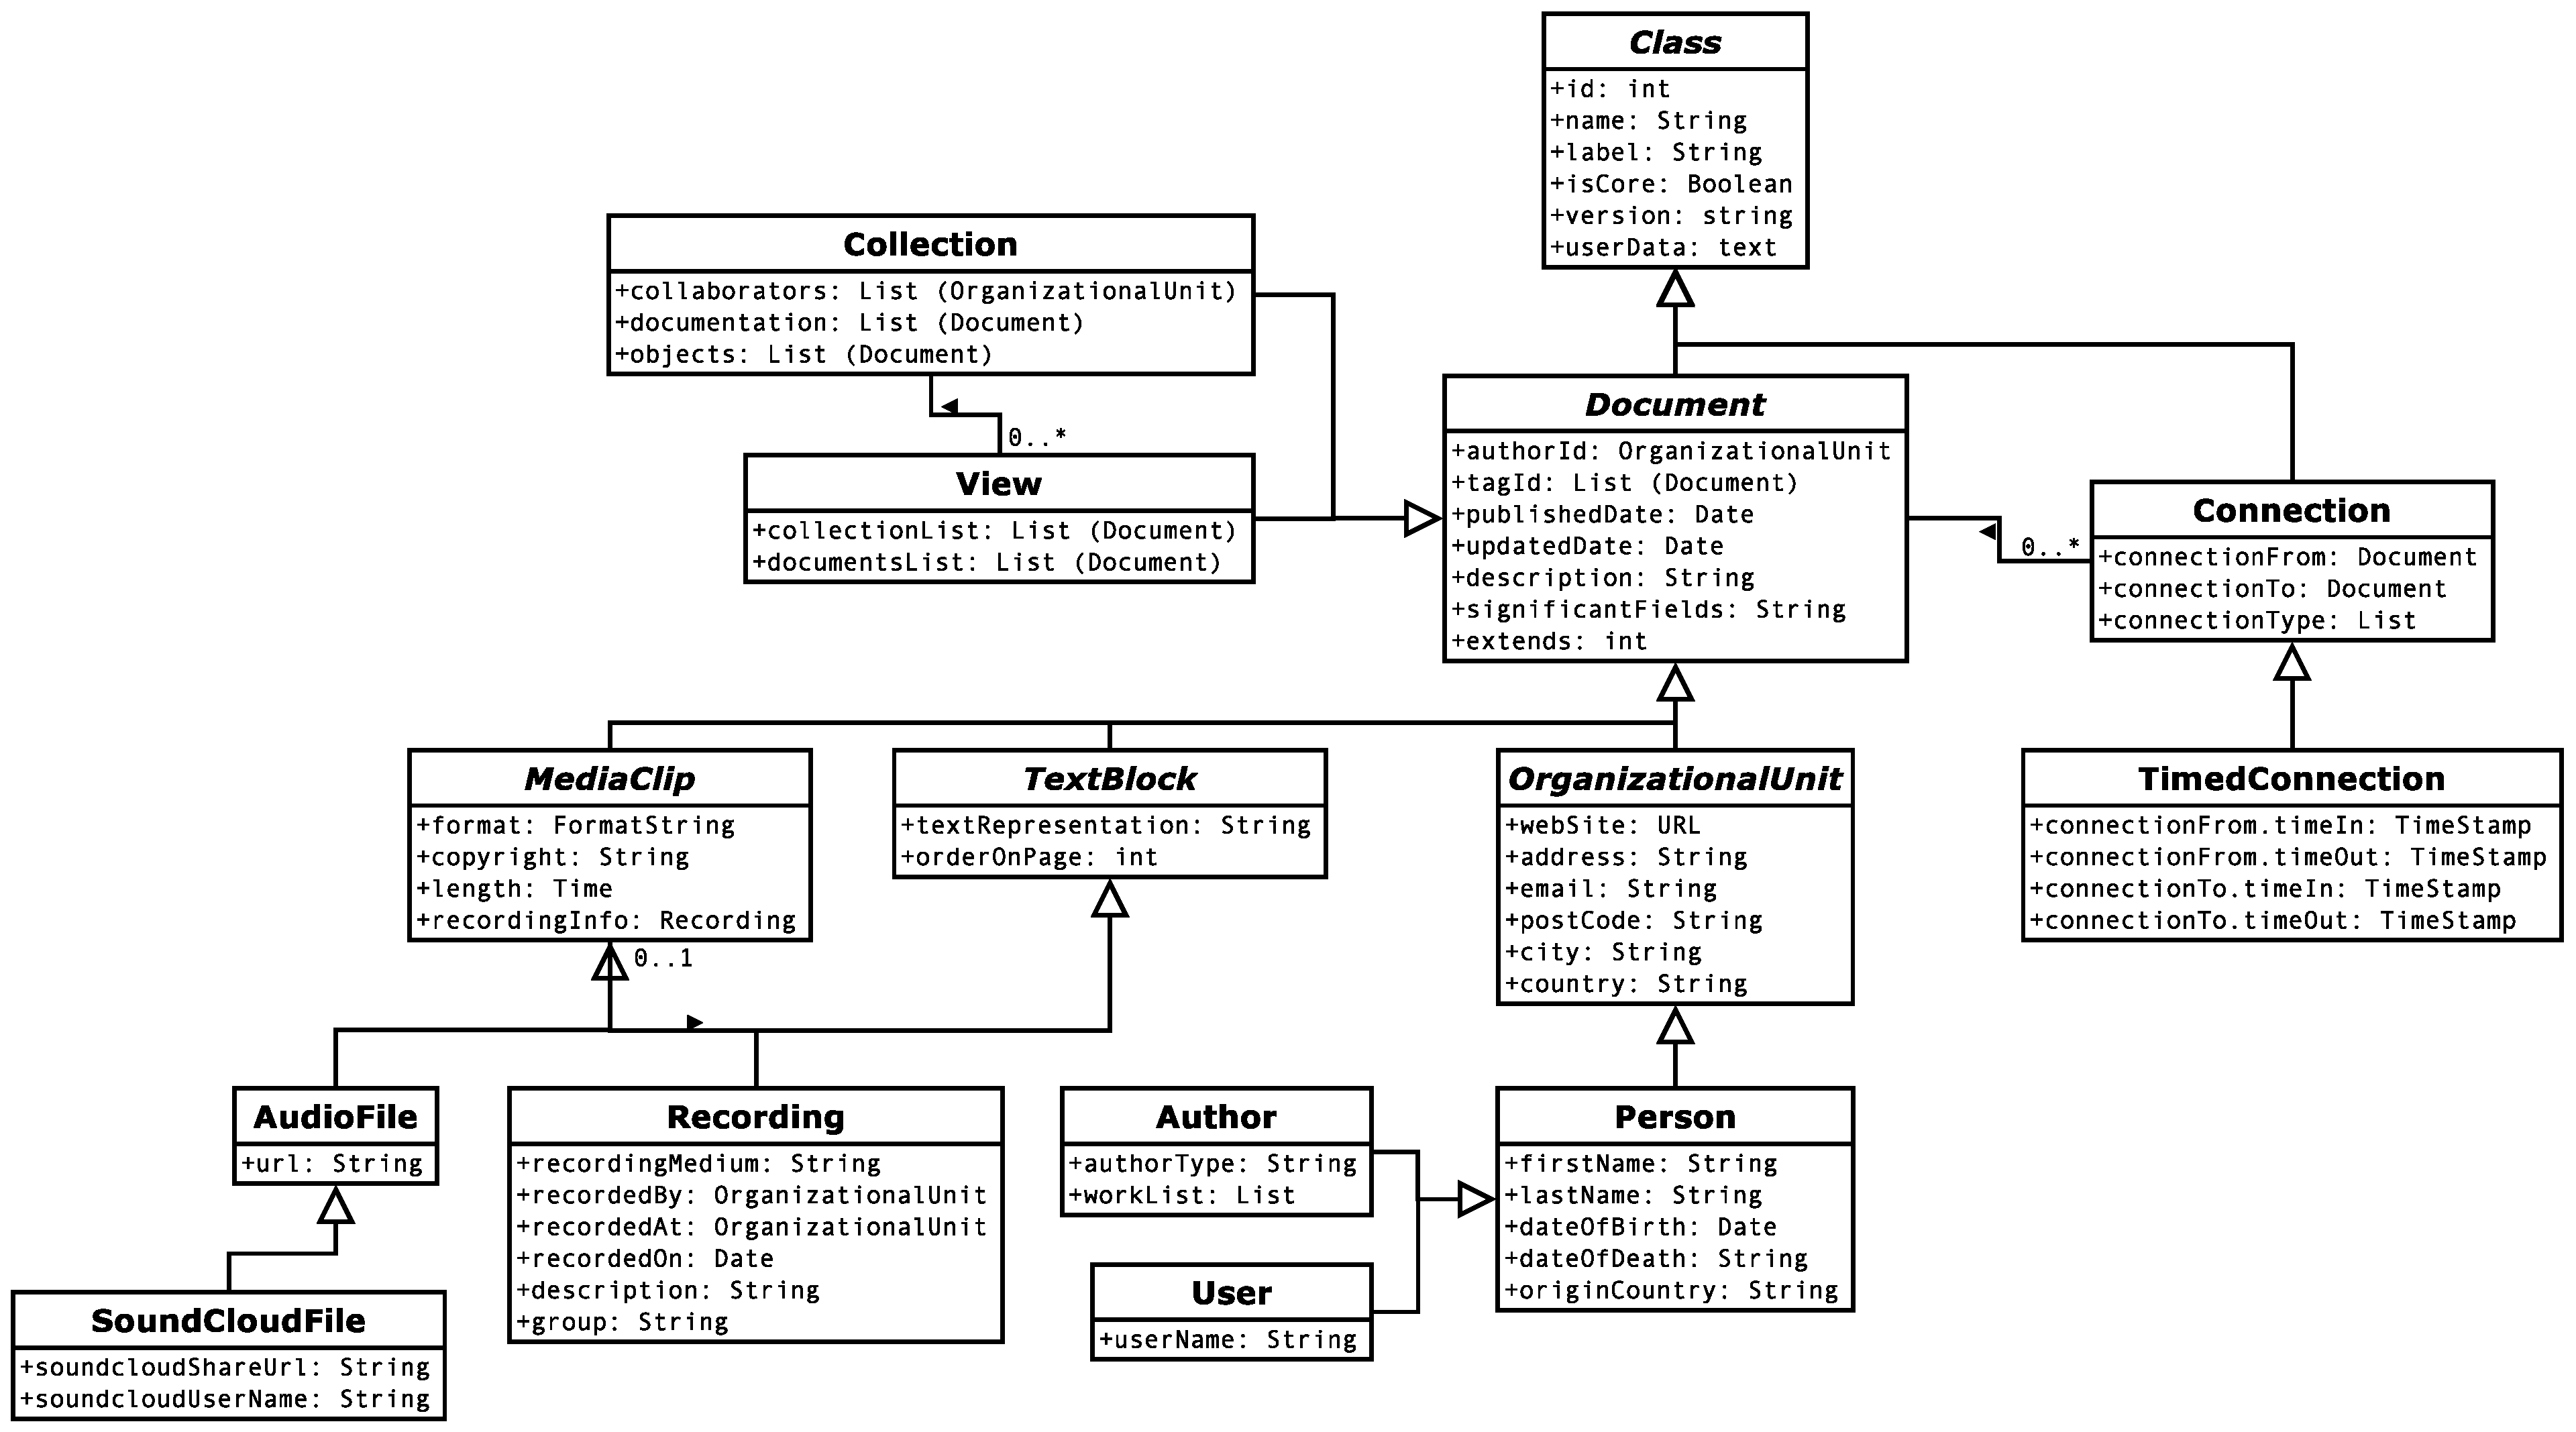
\includegraphics[height=6.7cm]{img/classdiagram-2018-sub.eps}
\caption{A part of the diagram for the latest version of the class hierarchy for the documentation system ArtDoc. All classes extend the base class \emph{Class} and most classes also extend the \emph{Document} class. This allows for new and more specialized classes to be easily added.}
\label{fig:example}
\end{figure}

\section{The Archive}
\label{sec:archive}
The structure of the archive is a set of classes that represent different kinds of resources and it is a feature of the system that classes can easily be added and extend the basic classes. There are a number of general, abstract, classes that serve as templates for further specialized classes. For example, the two base classes that most other classes inherit from are the \emph{Class} and \emph{Document} classes (see Figure \ref{fig:example}). As a consequence a reference of the type \emph{Document} can point to almost any kind of resource in the archive, and all instances of any type that are children of these classes will have the same basic set of attributes. Similarly, an \emph{OrganizationalUnit} is the base class for all kinds of references to \emph{Persons}, \emph{Users} or \emph{Authors}. A \emph{Collection} is a means for grouping resources together, for example as a convenience when several users collaborate on a project, and a \emph{View} is a presentation of a list of one or more such collections.

One of the fundamental properties of this experimental documentation archive is the \emph{Connection} class. It defines a connection between two instances and the principle is that it should be possible to connect anything to anything -- that is any \emph{Document} may be connected to any other \emph{Document}. In this way connected objects can create a semantic web where the kinds of connections, as well as the number of connections, gives the user information about the documented data. Hence, connections give meaning to instances, and instances can further be understood through the number of connections they have. In this way, even after the raw data has been entered and connections have been made, the archive becomes a method in its own right. Furthermore, connections of the type \emph{TimedConnection} can point to a specific point in time, or a range, in an instance that documents some kind of time based data such as an audio or video file.

All classes are defined in an XML description which acts as a template for all instances of that particular type, adding in the attributes of all parent classes. Below is an example of the definition of the \emph{Connection} class (some information is stripped out for legibility). The instance attributes are defined within the \emph{attributes} tag.
\medskip

\noindent
{\it Example of a class definition}
\begin{verbatim}
<Class xmlns:xsi="http://www.w3.org/2001/XMLSchema-instance">
    <class-name>Connection</class-name>
    <parent>Class</parent>
    <class-description>A child class to Class describing a 
     connection between two nodes within the system. The id of the 
     connected classes are the references.
    </class-description>
    <documentation/>
    <attributes>
        <connection-from type="Ref" ref-class="Document" 
                         desc="Connection from" edit="1" 
                         required="1" doc="The reference to the 
                         document that connects another document. />
        <connection-to type="Ref" ref-class="Document" 
                       desc="Connection to" edit="1" 
                       required="1" doc="The reference to the 
                       document that is connected."/>
        <connection-type type="String" desc="Type of connection" 
                         edit="1" required="0"/>
    </attributes>
</Class>
\end{verbatim}
\noindent
{\small (Example class definition for the \emph{Connection} class. As can be seen the definition contains documentation strings for both the class and for each of the attributes. The 'type' and 'required' parameters of each attribute allows for basic validation of an instance.)}

\vspace{0.5cm}

The design principle has been to keep classes small and particular, and as mentioned above, it should be possible to add new classes to the system simply by adding new class definitions that inherit existing classes. However, more complicated and specialized classes may obviously require additional definitions on either the client or the server, or both. For example, a video class that allows the user to add a video through an external service may depend on a particular API for which support needs to be added. 

Using abstract classes as basic types for the data allows the implementation of simple and generic widgets in the user interface. For example, the \emph{MediaClip} class serves any sub-classes with basic functionality for playing back an audio or video file with a generic set of playback functions. Implementing support for a class that extends this base class, such as YouTube or similar, may then be limited to supplying a wrapper that maps the base class functionality to the extended class' API. Though the system could easily be made to support that routines needed for a particular class be added in the class definition, this may introduce security issues that needs to be considered.

The development of an implementation of ArtDoc is currently progressing using eXist db \cite{exist} as the backend using XQuery for the server side scripts, and a web client as front end (see Figure \ref{fig:client}). Apart from the goal to document \emph{Repetition Repeats all other Repetitions} ArtDoc will be tested as a documentation database for works performed in the \emph{Klangdome} at the Royal College of Music in Stockholm. The \emph{Klangdome}, situated in one of the concert halls is a flexible system of up to 49 loudspeakers in a dome like configuration that affords a platform for a wide variety of scientific and artistic projects. The attempt to document the works performed offers a challenging task for ArtDoc that will guide its future development.

Finally, ArtDoc will be used in a newly initiated research project under the headline of \emph{Musical Transformations}. \emph{Musical Transformations} brings researchers in ethnomusicology and artistic research in music together in order to develop new knowledge and deepened understanding of processes of renewal of musical practices in intercultural and transnational contexts. Musical traditions in Vietnam and in Sweden will be documented and new interdisciplinary methods for research into creative processes in music will be developed in which ArtDoc will play an important role.
\begin{figure}
\centering
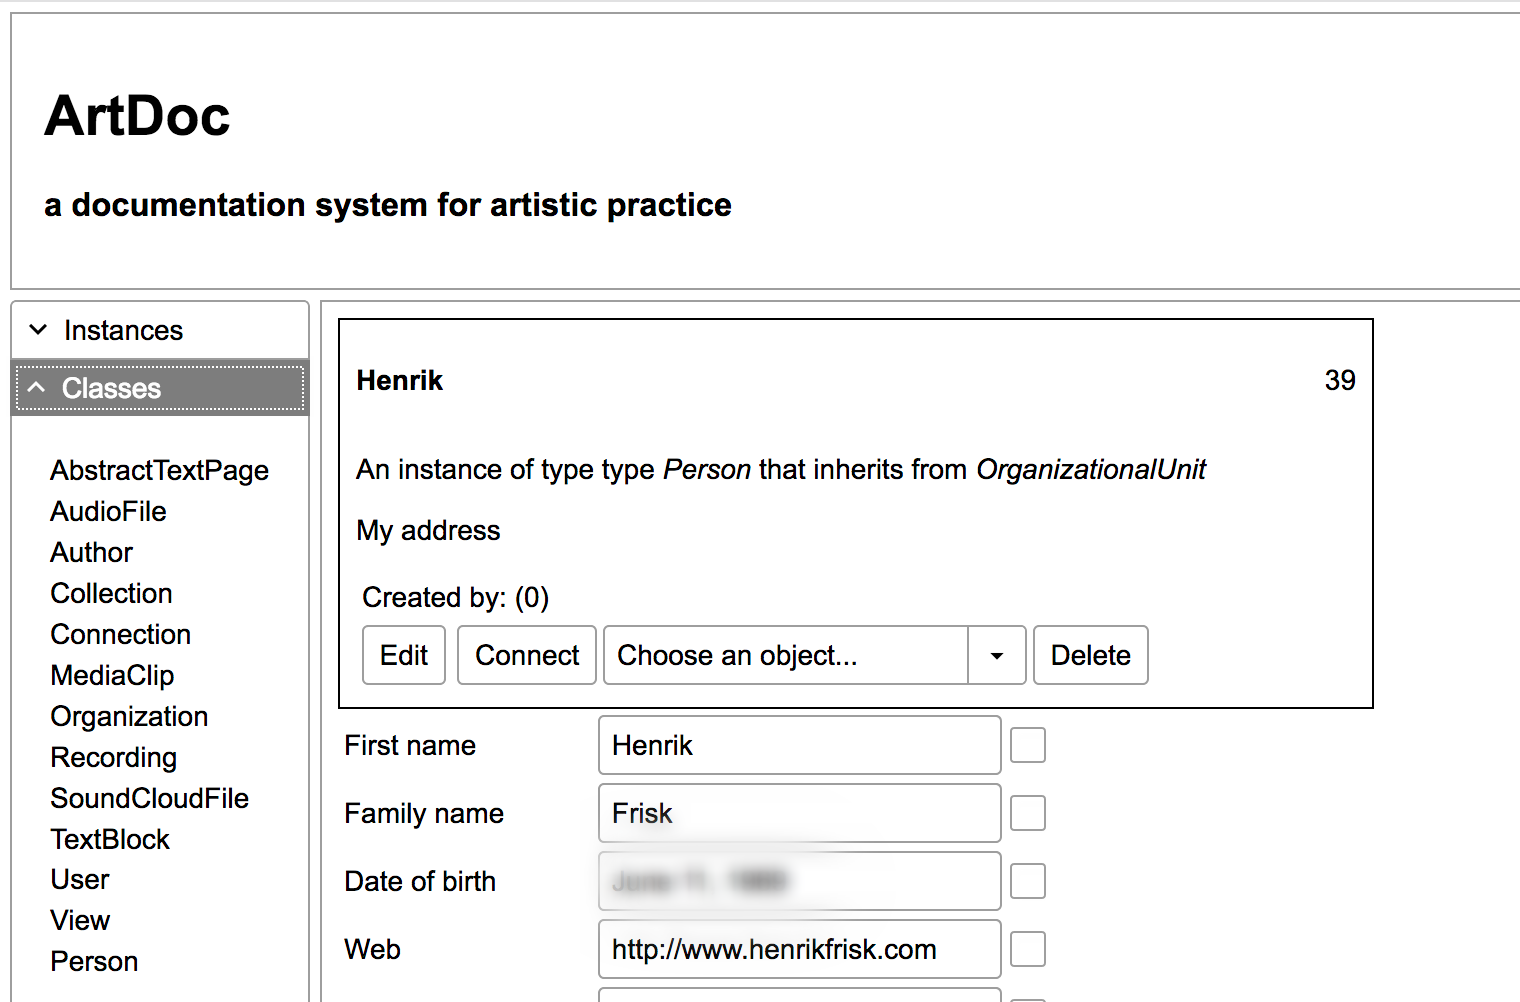
\includegraphics[height=7cm]{img/screen-dump.png}
\caption{A screen dump from an early and preliminary version of the interface to ArtDoc. To the right are a list of instantiable classes and in the main view is an item of the type \emph{Person} open for editing.}
\label{fig:client}
\end{figure}


\section{Discussion}
\label{sec:discussion}
The question of how to best document the creative forces that digital technology allows for is without doubt one of the important challenges in the near future. Though this is a question that has bearing on almost all aspects of social life in the 21st century, in the case of artistic practice in music there are a few important considerations that are of particular interest. First, there is the risk that the nearly ubiquitous digital domain negatively influences the willingness to invest in an active listening process. Though there is little that actually points in this direction, if anything listening to live music appears to have increased in urban areas, the convenience of online music services that delivers exactly the music it thinks we want to hear is intimidating at times. The materiality of music production in the widest sense is not necessarily encoded into the digital representation of music. Secondly, the incredible digital tools that we have at hand may make visible aspects of musical composition and performance in new and interesting ways. Collecting audio and video documentation, for example, has never been easier, but the massive amounts of data that it generates can be daunting without a structured method. These are only two of many facets of the changes that digitization affords, but if these are addressed in a way that bring forth the conditions of musical practice they may provide interesting opportunities for the development of artistic practices. When the focus moves from the result to the processes prior to the result, the view on the musical work is likely to also change. 

If it proves effective there are a number of ways in which it can be expanded. For example, currently ArtDoc is largely a single user application that offers musicians and composers to document their own work. However, its real strength will show when users can interact on projects together. The driving force in the development has been my own need for a tool to both document my work, but also to allow for a more efficient way to interact with my colleagues on projects. The basic ability to control access to individual items in the archive through permissions is already in place. Furthermore, the functionality that the classes \emph{Collection} and \emph{View} offer can with some modification turn the archive into a proper presentation tool, or even a tool for performance, in its own right.

In this short overview I have tried to argue for the need for new strategies for the documentation of artistic practice, as well as presented an experimental tool to meet these demands. A modular system with a hierarchy of documentation classes, an archive and a user client to enter and access data is under development and preliminary tests have been carried out. The primary purpose of ArtDoc, however, is to explore the various ways in which a documentation of an artistic practice can be carried out that provides meaningful information to both the artist and the listener.


\subsubsection*{Acknowledgments.} With acknowledgments to my colleague Jamie Bullock and the other contributors of the Integra project.
\hyphenation{Post-Script}
\begin{thebibliography}{10}

\bibitem{rc2017}
About the research catalogue, \url{https://www.researchcatalogue.net/portal/about}
\newblock Web resource (2017)
\newblock Accessed May 15, 2017.

\bibitem{Bachimont2003}
Bachimont, B., Blanchette, J.-F., Gerzso, A., Swetland, A., Lescurieux, J.-F.,
  Morizet-Mahoudeaux P., Donin, N. and Teasley, J.:
\newblock Preserving Interactive Digital Music: a Report on the MUSTICA
  Research Initiative.
\newblock In {\em Proceedings. Third International Conference on Web Delivering
  of Music.Web Delivering of Music}. WEDELMUSIC (2003)

\bibitem{biggs10}
Biggs, M., Karlsson, H., (eds).:
\newblock {\em The Routledge Companion to Research in the Arts}.
\newblock Routledge, London (2010)

\bibitem{bullock06}
Bullock, J., Coccioli, C.:
\newblock {Modernising Musical Works Involving Yamaha DX-based Synthesis: a
  Case Study}.
\newblock {\em Organised Sound}, 11(3) (2006)

\bibitem{frisk-bull07}
Bullock, J., Frisk, H.:
\newblock {libIntegra: A System for Software-Independent Multimedia Module
  Description and Storage}.
\newblock In {\em Proceedings of the International Computer Music Conference
  2007}, Copenhagen, Denmark (2007)

\bibitem{frisk09}
Bullock, J., Frisk, H.:
\newblock An Object Oriented Model for the Representation of Temporal Data in
  the Integra Framework.
\newblock In {\em Proceedings of the International Computer Music Conference
  2009}. ICMA (2009)

\bibitem{frisk-bullock08}
Bullock, J., Frisk, H., Coccioli, L.:
\newblock Sustainability of `Live Electronic' Music in the Integra Project.
\newblock In {\em {The 14th IEEE Mediterranean Electrotechnical Conference
  Proceedings}}, Ajaccio, Corsica (2008)

\bibitem{cuervo2011}
Cuervo, A. P.:
\newblock {Preserving the Electroacoustic Music Legacy: A Case Study of the
  Sal-Mar Construction at the University of Illinois}.
\newblock {\em Notes.}, 68(1):33--47 (2011)

\bibitem{Douglas2007}
Douglas, J.:
\newblock {General Study 03 Final Report : Preserving Interactive Digital
  Music}.
\newblock Technical report, The MUSTICA Initiative (2007)

\bibitem{eco68}
Eco, U.:
\newblock {\em The Open Work}.
\newblock Hutchinson Radius, London (1968)
\newblock (English translation published in 1989)

\bibitem{Folkestad1997}
Folkestad, G., Lindstr\"{o}m, B., Hargreaves, D.~J.:
\newblock Young People's Music in the Digital Age: A Study of Computer Based
  Creative Music Making.
\newblock {\em Research Studies in Music Education}, 9(1):1--12 (1997)

\bibitem{frisk08}
H.~Frisk.:
\newblock {\em Improvisation, Computers and Interaction: Rethinking
  Human-Computer Interaction Through Music}.
\newblock PhD thesis, Faculty of Fine and Performing Arts, Lund University (2008)

\bibitem{frisk2018}
Frisk, H.:
\newblock The Archive that Writes Itself.
\newblock {\em SMC} (2018)
\newblock In print.

\bibitem{frisk-ost06}
Frisk, H., \"{O}stersj\"{o}, S.:
\newblock Negotiating the Musical Work. An Empirical Study.
\newblock In: {\em Proceedings of the International Computer Music Conference
  2006}, pp. 242-249. ICMA, San Francisco, Calif.: Computer Music Assoc.,
  (2006)

\bibitem{frisk-ost06-2}
Frisk, H., \"{O}stersj\"{o}, S.:
\newblock Negotiating the musical work. {A}n Empirical Study on the
  Inter-Relation Between Composition, Interpretation and Performance.
\newblock In: {\em Proceedings of EMS -06, Beijing. Terminology and
  Translation}. Electroacoustic Music Studies, EMS (2006)

\bibitem {friskcoessens2013}
  Frisk, H., Coessens, C., \"Ostersj\"o, S.: Repetition,
  resonance and discernment. In D. Crispin, B. Gilmore (Eds.),
  Artistic Experimentation in Music (pp. ). : Orpheus Institute
  Series, Gent (2014)

\bibitem{ostersjo08}
\"{O}stersj\"{o}, S.:
\newblock {\em SHUT UP `N' PLAY! Negotiating the Musical Work}.
\newblock PhD thesis, Malm\"{o} Academy of Music, Lund University (2008)

\bibitem{Roeder2006}
Roeder, J.:
\newblock {Authenticity of Digital Music : Key Insights from Interviews in the
  MUSTICA Project}.
\newblock Technical report, The MUSTICA Initiative (2006)

\bibitem{integra} IntegraLab, \url{http://integra.io/}
\bibitem{exist} eXist db, \url{http://exist-db.org}
\end{thebibliography}

\end{document}
